\begin{pastexam}[label={px:ncku-106-prog-01}]{成大資訊聯招 106 學年度 第 1 題}
（問答）

(10\%) Given inorder and preorder traversal of a tree as follows.\\
inorder: JHKFIDGBEAC\\
preorder: ABDFHJKIGEC\\
(5\%) reconstruct the binary tree\\
(5\%) show the postorder traversal of this tree
\end{pastexam}

\begin{pastsoln}
答案：後序是 JKHIFGDEBCA，樹畫在下面。

節點名稱都不同，前序加中序可以唯一決定一棵二元樹（資結書定理~7.4）。 做法（資結書第~7.4~節）：
前序的第一個字是根；在中序裡找到根，左邊是左子樹的中序、右邊是右子樹的中序；左子樹有幾個節點，前序
在根後面就取幾個當左子樹的前序，剩下的是右子樹的前序。 對每棵子樹重複。

\begin{center}
\small
\begin{tabular}{lllll}
\toprule
前序 & 中序 & 根 & 左子樹（中序） & 右子樹（中序） \\
\midrule
ABDFHJKIGEC & JHKFIDGBE\,A\,C & A & JHKFIDGBE（9 個） & C \\
BDFHJKIGE & JHKFIDG\,B\,E & B & JHKFIDG（7 個） & E \\
DFHJKIG & JHKFI\,D\,G & D & JHKFI（5 個） & G \\
FHJKI & JHK\,F\,I & F & JHK（3 個） & I \\
HJK & J\,H\,K & H & J & K \\
\bottomrule
\end{tabular}
\end{center}

每一列的前序都是上一列「根後面取左子樹個數」得到的，例如第一列根 A 的左子樹有 9 個節點，前序取 A 後面
9 個字 BDFHJKIGE；剩下的 C 是右子樹。 只剩一個字的子樹（C、E、G、I、J、K）就是葉節點。

\begin{center}
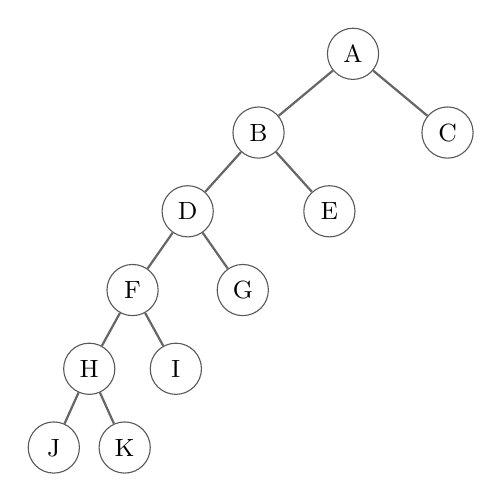
\begin{tikzpicture}[
    btn/.style={circle, draw=black!65, line width=0.4pt, minimum size=6.5mm, inner sep=0pt, font=\small},
    level distance=10mm, edge from parent/.style={draw=black!60, thick},
    level 1/.style={sibling distance=24mm}, level 2/.style={sibling distance=18mm},
    level 3/.style={sibling distance=14mm}, level 4/.style={sibling distance=11mm},
    level 5/.style={sibling distance=9mm}]
\node[btn] {A}
    child {node[btn] {B}
        child {node[btn] {D}
            child {node[btn] {F}
                child {node[btn] {H}
                    child {node[btn] {J}}
                    child {node[btn] {K}}}
                child {node[btn] {I}}}
            child {node[btn] {G}}}
        child {node[btn] {E}}}
    child {node[btn] {C}};
\end{tikzpicture}
\end{center}

\textbf{後序}（左、右、根）：從最深的 H 子樹開始，J、K、H；接著 F 的右子節點 I，再 F；D 的右子節點 G，
再 D；B 的右子節點 E，再 B；根的右子節點 C，最後 A。 得到
\[
\text{J K H I F G D E B C A}.
\]
核對：這棵樹的中序是 J H K F I D G B E A C、前序是 A B D F H J K I G E C，和題目給的一樣。
\end{pastsoln}
